\appendix

\chapter{\faBook\ \hspace{0.3cm} Manual de usuario de la aplicación}
\label{app:manual}

\vspace{-1cm}
\begin{center}
\LARGE{ATC Analysis and Training Tool}
\end{center}

\bigskip

\subsection*{\faInfoCircle\ \hspace{0.3cm} Información de la aplicación}

La aplicación ha sido desarrollada en el contexto del Trabajo Fin de Grado del plan de estudios del Grado en Ingeniería Aeroespacial en Aeronavegación de la Universidad Rey Juan Carlos, 

\begin{description}
\item \faPlay\ \hspace{0.4cm} Ejecutable para Microsoft Windows (x64)
\item \faUser\ \hspace{0.4cm} Jaime Valle Alonso
\item \faCalendar\ \hspace{0.3cm} Versión 1.2 (2025).
\end{description}



\subsection*{\faGear\ \hspace{0.3cm} Instalación y ejecución}

No es necesaria su instalación, basta con seguir los siguientes pasos:

\begin{enumerate}
\item Descomprimir el fichero \textit{2025-07-02 - Windows Intel 64-bit v1.2.zip}.

\item Entrar al directorio \textit{Windows Intel 64-bit}.

\item Ejecutar el fichero \textit{ATC Analysis and Training Tool.exe}.
\end{enumerate}

\begin{figure}[!hbtp]
	\centering
	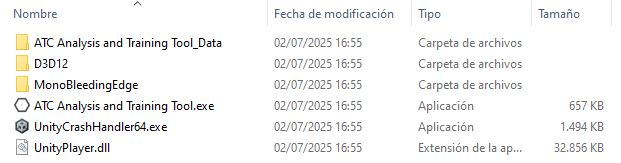
\includegraphics[width=0.9\linewidth]{images/content/AppExe.jpg}
	\caption*{\vspace*{-0.5cm}Fichero ejecutable y resto de archivos de la aplicación.}
	\label{fig:AppExe}
\end{figure}



\clearpage

\begin{landscape}

\subsection*{\faGlobe\ \hspace{0.3cm} Pantalla radar}

\begin{figure}[!hbtp]
	%\centering
	\hspace{-1cm}
	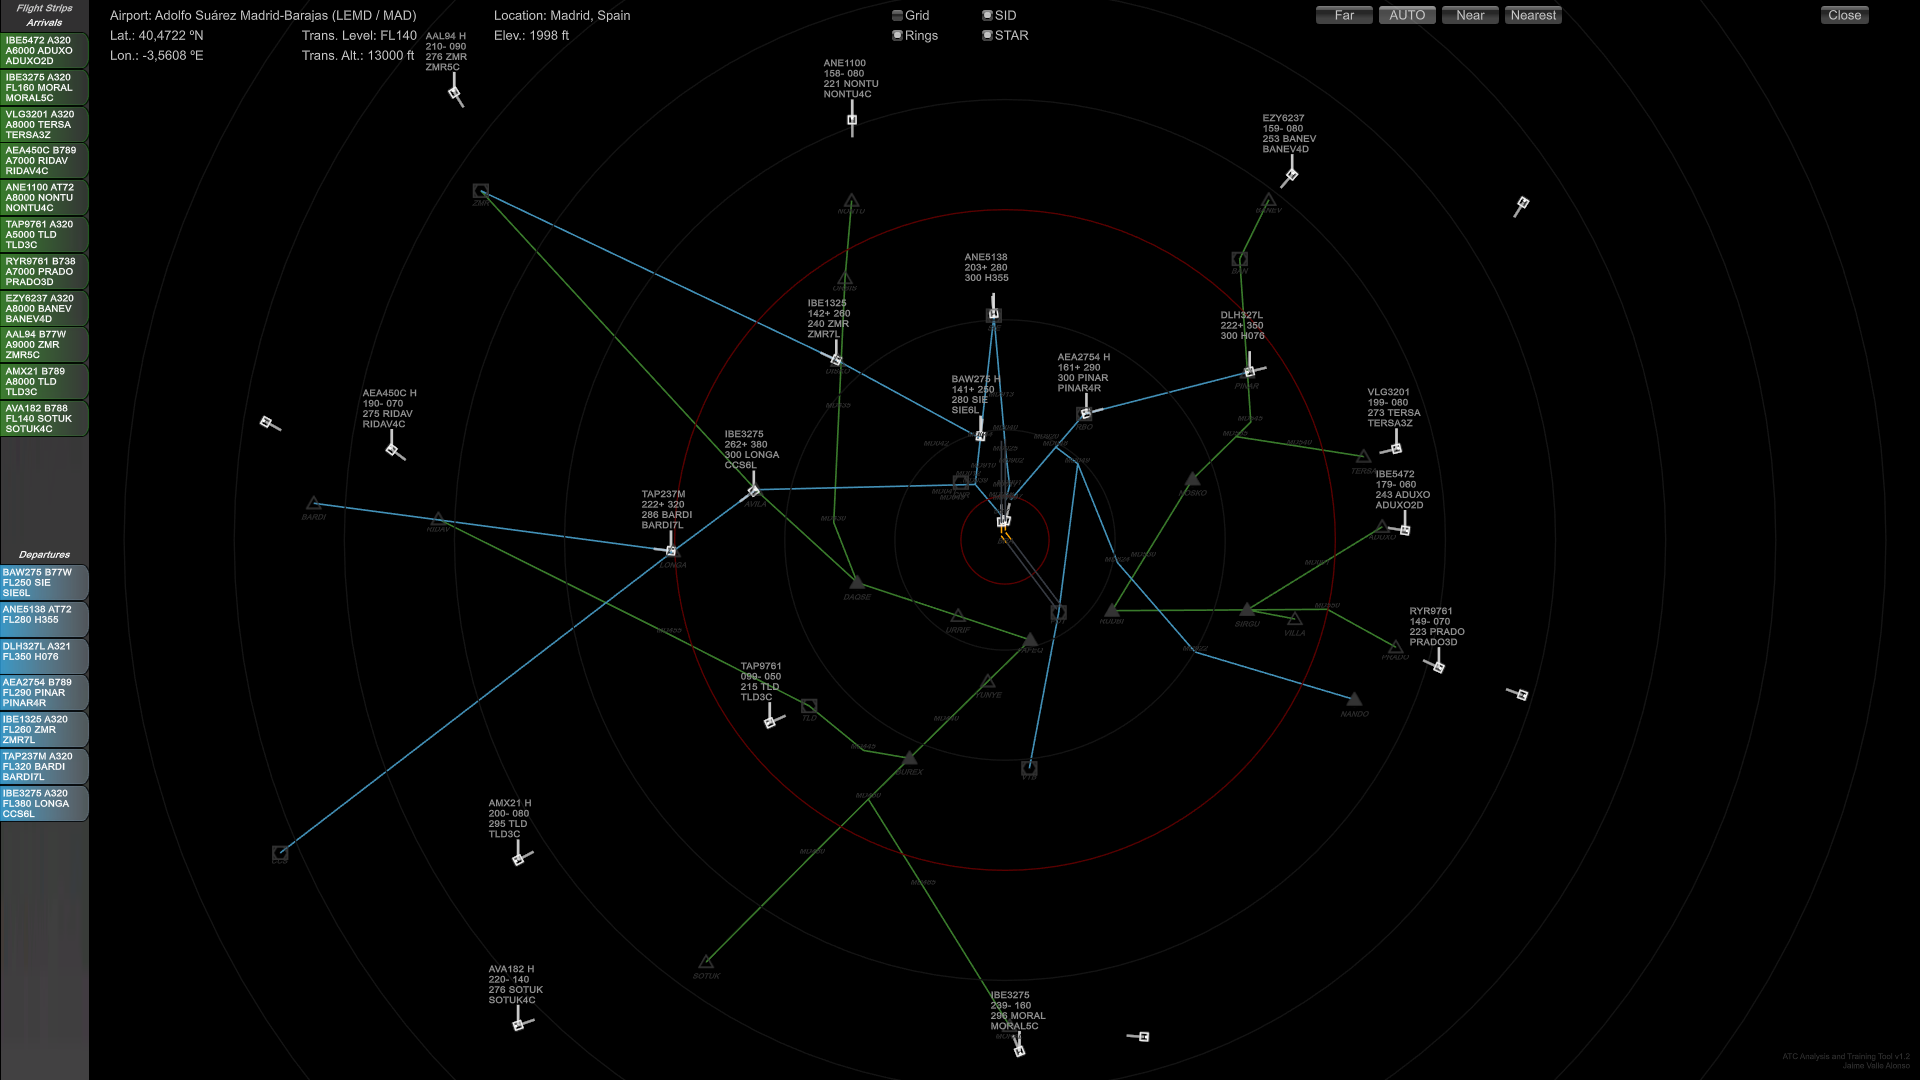
\includegraphics[width=1.0\linewidth]{images/content/Aplicacion1080.png}
	\caption*{Vista principal de la aplicación.}
	\label{fig:Aplicacion1080}
\end{figure}
\end{landscape}






\clearpage

\subsection*{\faTag\ \hspace{0.3cm} Panel de fichas de progreso de vuelo}

En el panel izquierdo se muestran las fichas de progreso de vuelo. Se tiene una ficha por cada uno de los tráficos que se están siendo controlados, categorizados por llegadas (\textit{arrivals}) y salidas (\textit{departures}). Contienen la información esencial de ese vuelo:

\begin{figure}[!hbtp]
	\centering
	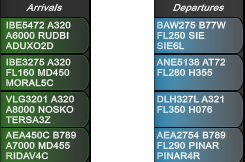
\includegraphics[width=0.5\linewidth]{images/app/FlightStrips.png}
	\caption*{Fichas de progresión de vuelo de llegadas y salidas.}
\end{figure}

La información que contiene es la siguiente:

\begin{itemize}
\item Identificador compuesto por código OACI de la compañia seguido del número de vuelo.

\item El código OACI/ICAO del tipo de avión.

\item La altitud actual en cientos de pies seguido del signo (-) si la aeronave está descenciendo, (+) si está ascendiendo o (=) si está manteniendo la altitud.

\item La altitud autorizada en cientos de pies.

\item La actual velocidad en nudos.

\item El siguiente punto de ruta autorizado.

\item El procedimiento estándar al que pertenece el siguiente punto de ruta (puede estar vacío).
\end{itemize}


\clearpage

\subsection*{\faInfo\ \hspace{0.5cm} Etiqueta de datos de la aeronave}

Al lado de cada aeronave aparece su etiqueta de datos, la cual puede cambiarse de posición haciendo clic con el botón izquierdo del ratón encima de la aeronave. Hay seis posibles posiciones que van rotando en el sentido de las agujas del reloj por cada pulsación.

\begin{figure}[!hbtp]
	\centering
	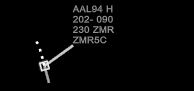
\includegraphics[width=0.5\linewidth]{images/app/Etiqueta.png}
	\caption*{Etiqueta de datos de la aeronave.}
\end{figure}

\begin{itemize}
\item Identificador compuesto por código OACI de la compañia seguido del número de vuelo.

\item Si la aeronaves es de categoría \textit{Heavy}, se mostrará una (H) después del número de vuelo.

\item La altitud (A) o nivel de vuelo (FL) autorizado en la última consigna.

\item El siguiente punto de ruta autorizado.

\item El procedimiento estándar al que pertenece el siguiente punto de ruta (puede estar vacío).
\end{itemize}



\subsection*{\faTerminal\ \hspace{0.5cm} Zona de texto de comunicaciones}

Las asignaciones que el ATC realiza a las aeronaves se muestran en la franja inferior de la pantalla radar. A la izquierda aparecen los comandos ATC, mientras que a la derecha las aeronaves.

\begin{figure}[!hbtp]
	\centering
	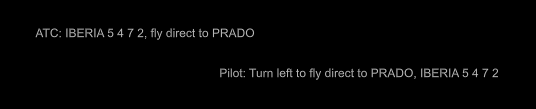
\includegraphics[width=1.0\linewidth]{images/app/ComunicacionATC2.png}
	\caption*{Zona de texto de comunicaciones.}
\end{figure}



Del mismo modo, si una aeronave sobrevuela un punto de notificación obligatoria (\textit{compulsory}), también se notificará ahí.

\begin{figure}[!hbtp]
	\centering
	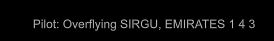
\includegraphics[width=0.5\linewidth]{images/app/Overflying.png}
	\caption*{Reporte de sobrevuelo.}
\end{figure}



\clearpage

\subsection*{\faHandORight \hspace{0.3cm} Interacción con las aeronaves}

Para interactuar con las aeronaves debe situarse el ratón encima de la aeronave interesada y hacer clic derecho con el ratón. Si la aeronave ya está siendo controlada por el usuario se desplegára el menú de control ATC, en caso contrario aparecerá la opción <<\textit{Contact}>>.

\begin{figure}[!hbtp]
	\centering
	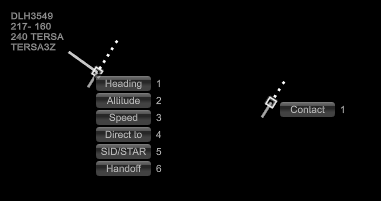
\includegraphics[height=6cm]{images/app/MenuControlATC.png}
	\caption*{Menú de control ATC para tráficos controlados y aún sin controlar.}
\end{figure}




\clearpage

\subsubsection*{Comando de rumbo}

Una vez desplegado el menú de control ATC y mientras se visualiza éste, puede pulsarse la opción <<Heading>> o pulsar la tecla <<1>> del teclado y se desplegará el submenú de asignación de rumbo. 

Por defecto, al abrirse el submenú aparecerá relleno el rumbo actual de la aeronave. Puede modificarse el valor de los campos pulsando sobre las flechas inferiores y superiores de cada dígito o escribiendo directamente la cifra numérica con el teclado. 

\begin{figure}[!hbtp]
	\centering
	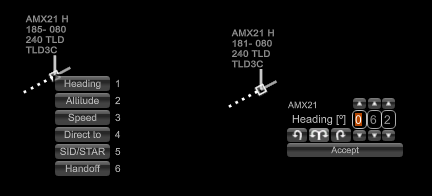
\includegraphics[width=\linewidth]{images/app/SubmenuHeading.png}
	\caption*{Menú de control ATC y submenú para instruir rumbo (\textit{heading}).}
\end{figure}

Los rumbos admisibles son del \texttt{0 0 1} al \texttt{3 6 0}.

Además, se puede forzar a realizar el viraje a izquierdas, derechas o dejar a la aeronave que eliga según el que menor distancia angular presente. 

Para hacer efectivo el comando puede presionarse el botón <<Accept>> o pulsar \texttt{Intro}.



\clearpage

\subsubsection*{Comando de altitud}

Una vez desplegado el menú de control ATC y mientras se visualiza éste, puede pulsarse la opción <<Altitude>> o pulsar la tecla <<2>> del teclado y se desplegará el submenú de asignación de altitud. 

Por defecto, al abrirse el submenú aparecerá relleno la altitud actual de la aeronave en pies. Puede modificarse el valor de los campos pulsando sobre las flechas inferiores y superiores de cada dígito o escribiendo directamente la cifra numérica con el teclado. 

\begin{figure}[!hbtp]
	\centering
	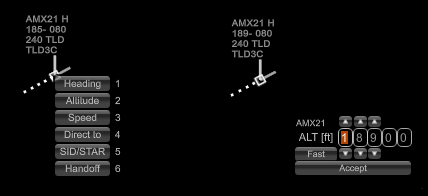
\includegraphics[width=\linewidth]{images/app/SubmenuAltitude.png}
	\caption*{Menú de control ATC y submenú para instruir altitud (\textit{altitude}).}
\end{figure}

Se introducirá la altitud de consigna en cientos de pies, es decir, en niveles de vuelo, ya que no tiene sentido instruir altitudes que no sean múltiplos de 100. La altitud máxima admisible es de \SI{55000}{ft} (\texttt{5 5 0 0 0}).

Además, se puede solicitar a la aeronave que realice la maniobra lo más rápido posible mediante la pulsación del interruptor <<Fast>>. 

Para hacer efectivo el comando puede presionarse el botón <<Accept>> o pulsar \textit{Intro}, instruyéndose automáticamente al avión altitud o nivel de vuelo dependiendo de si la consigna está por encima o por debajo de la capa de transición.





\clearpage

\subsubsection*{Comando de velocidad}

Una vez desplegado el menú de control ATC y mientras se visualiza éste, puede pulsarse la opción <<\textit{Speed}>> o pulsar la tecla <<3>> del teclado y se desplegará el submenú de asignación de velocidad. 

Por defecto, al abrirse el submenú aparecerá relleno la velocidad actual de la aeronave en nudos. Puede modificarse el valor de los campos pulsando sobre las flechas inferiores y superiores de cada dígito o escribiendo directamente la cifra numérica con el teclado. 

\begin{figure}[!hbtp]
	\centering
	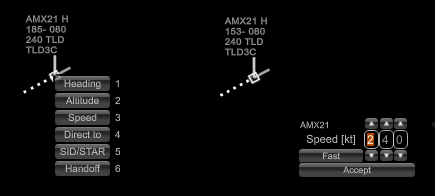
\includegraphics[width=\linewidth]{images/app/SubmenuSpeed.png}
	\caption*{Menú de control ATC y submenú para instruir velocidad (\textit{speed}).}
\end{figure}

Se introducirá la velocidad de consigna en nudos. La velocidad máxima admisible es de \SI{500}{kt} (\texttt{5 0 0}), mientras que la velocidad mínima está limitada a \SI{120}{kt} pero será la aeronave la que determine, según su categoría, cuál es la velocidad mínima que puede aceptar.

\begin{figure}[!hbtp]
	\centering
	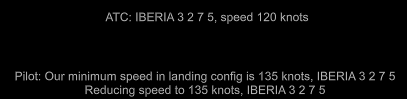
\includegraphics[width=0.85\linewidth]{images/app/ComunicacionATC.png}
	\caption*{La aeronave puede no aceptar velocidades de vuelo por debajo de un umbral.}
\end{figure}


Además, se puede solicitar a la aeronave que realice la maniobra lo más rápido posible mediante la pulsación del interruptor <<Fast>>. 

Para hacer efectivo el comando puede presionarse el botón <<Accept>> o pulsar \textit{Intro}.




\clearpage

\subsubsection*{Comando de vuelo directo a un punto}

Una vez desplegado el menú de control ATC y mientras se visualiza éste, puede pulsarse la opción <<\textit{Direct to}>> o pulsar la tecla <<4>> del teclado y se desplegará el submenú de vuelo directo a un punto. 

Aparecerá una lista deslizante con todos los puntos de navegación posibles, filtrados por fijos o radioayudas.  

\begin{figure}[!hbtp]
	\centering
	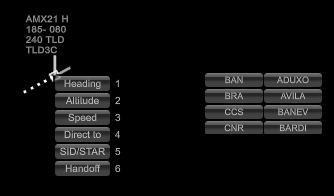
\includegraphics[width=0.8\linewidth]{images/app/SubmenuDirectTo.png}
	\caption*{Menú de control ATC y submenú para instruir volar directo a (\textit{direct to}).}
\end{figure}

Se seleccionará la opción que el usuario crea conveniente y automáticamente se instruirá el comando.





\clearpage

\subsubsection*{Comando de procedimiento estándar SID o STAR}

Una vez desplegado el menú de control ATC y mientras se visualiza éste, puede pulsarse la opción <<\textit{SID/STAR}>> o pulsar la tecla <<6>> del teclado y se desplegará el submenú de vuelo de procedimiento estándar de salida (SID) o de llegada (STAR). 

Aparecerá una lista deslizante con todos los procedimientos SID si el avión es una salida, o STAR si el avión es una llegada. Se seleccionará el procedimiento que se estime oportuno y aparecerá otro submenú con la lista de puntos secuenciales de ese procedimiento para definir el punto de entrada a la ruta.

\begin{figure}[!hbtp]
	\centering
	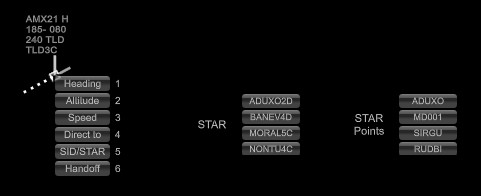
\includegraphics[width=\linewidth]{images/app/SubmenuProcedure.png}
	\caption*{Menú de control ATC y submenú para instruir procedimientos SID/STAR.}
\end{figure}

Se seleccionará la opción que el usuario crea conveniente y automáticamente se instruirá el comando.
